\documentclass{article}
\usepackage[preprint]{neurips_2025}
\usepackage[utf8]{inputenc}
\usepackage[T1]{fontenc}
\usepackage{amsmath,amssymb,booktabs,graphicx,microtype,array}
\usepackage[hidelinks]{hyperref}
\usepackage{url}
\newcommand{\Sys}{\mathcal{S}}
\raggedbottom
\title{Objective-Conditioned Design of Scientific Institutions}
\author{Anonymous authors\\Review-preparation draft\\Not submitted; target-cycle formatting pending}
\begin{document}
\maketitle
\begin{abstract}
What organizing system is selected when a scientific ecosystem's objective
changes? We make institutions executable design objects inside a persistent
researcher world: search can edit numerical parameters, algorithms, mechanisms
and process graphs while researcher-model weights and measurement functions
stay fixed. A finite, source-pinned study compares five proposal policies for
two objectives, retaining all 120 attempts, failures and exact ties. After
selection is frozen, 15 exact policies share 90 evaluations on five unused
two-year world seeds and a separate four-year diagnostic. Of 120 attempts, 64
complete, 25 fail generation and 31 fail execution. Throughput-selected
executable candidates and uniform numeric tuning match a hand-written
all-accept rule: mean 6.2 acceptances on the five unused seeds. A review-cost-sensitive
objective selects programs with no acceptances and fewer reviews, improving
the editable seed's mean loss from 2.58 to 1.92, but not the reviewer-free
reject-all reference's 0. All 64 completed specifications edit existing numeric
settings or selection source, not declared graph structure. An exercised
record-to-researcher input path motivates institutional analysis beyond
acceptance counts. These results separate objective-induced incentives,
permitted freedom, effective search and interface compliance; they do not
establish optimizer superiority, useful structural invention or real
scientific-policy benefit.
\end{abstract}

\section{Introduction}
Scientific institutions coordinate information, evaluation, resources and
opportunities. Rules affect what researchers encounter, attempt and submit
later. ScienceUtopia provides a persistent, literature-grounded LLM researcher
ecosystem for analyzing institutional interventions \citep{jin2026scienceutopia}.
We ask a different question: \emph{given an explicit objective, which organizing
system does a search process select, and through which executable changes?}
Search changes the institution, not researcher-model weights or a retrospectively
altered objective.

Evaluation is one possible mechanism, not a required centerpiece. Publication,
funding, governance, information routing, their absence and their connections
can also be design choices. Our executable space contains the original
researcher world rather than replacing it with a simpler differentiable toy.
Figure~\ref{fig:program} separates what may change from how search proposes changes.

\begin{figure}[t]
\centering
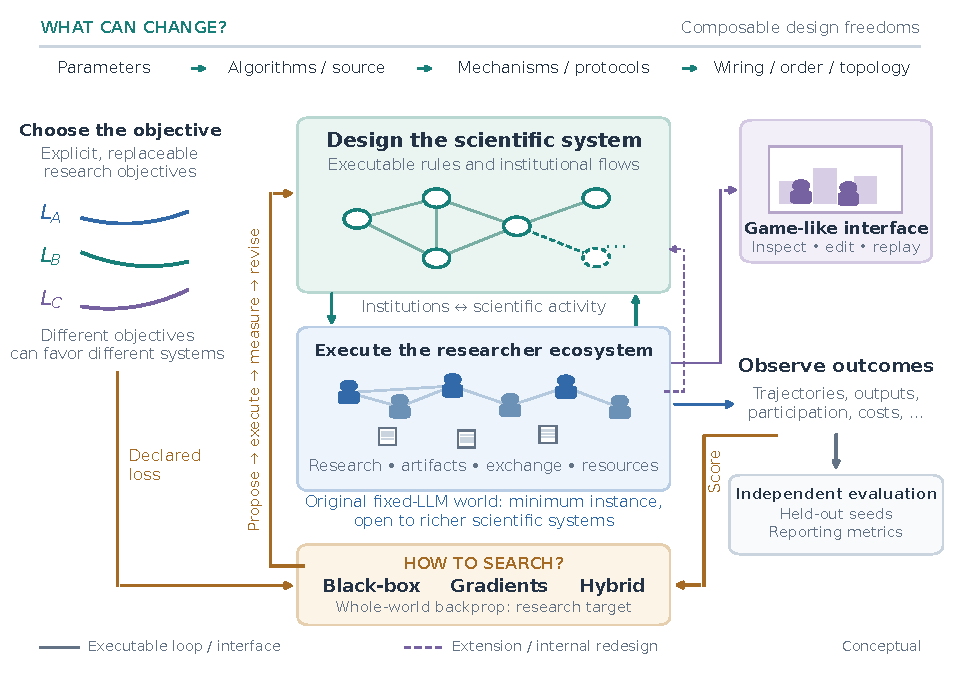
\includegraphics[width=\linewidth]{figures/program-concept/science-system-design-program.pdf}
\caption{\textbf{Scientific systems as design objects.} Parameters, algorithms,
mechanisms and wiring/processes are composable freedoms, not four optimization
methods. The objective and proposer are separate axes. This conceptual program
diagram does not show that every freedom was exploited in the finite study;
full-world differentiation and recursive improvement are not established.}
\label{fig:program}
\end{figure}

Neither LLM code generation nor simulated social optimization is new
\citep{liu2025mechanism,yang2024opro,zheng2020economist,zhuge2024gptswarm}.
Our contribution is the scientific-system design formulation and an audited
end-to-end comparison of objectives, proposal spaces and consequences.
\emph{Permission to edit a graph is not evidence of structural invention;
weak-seed improvement is not evidence of value beyond obvious rules.} We
therefore retain failures/ties, stronger references, unused conditions and
actual institution-to-researcher evidence.

\section{Executable scientific-system design}
Let $S\in\Sys$ be a scientific-system specification, $W$ fixed researcher weights,
$D$ a fixed corpus and $\xi$ a world condition. A trajectory is
$\tau\sim P(\cdot\mid S,W,D,\xi)$ and measurements are $M(\tau)$. For objective $\lambda$,
\begin{equation}
 \min_{S\in\Sys} J_\lambda(S)=\mathbb{E}_{\xi,\tau}[\ell_\lambda(M(\tau))].
\end{equation}
Finite observations identify neither a global optimum nor an exact expectation.
Fixed weights do not mean fixed behavior: institutional inputs can change
researcher responses and future states.

Typed SystemSpecs expose numerical settings, executable mappings/state updates,
mechanisms with ports, and wiring/schedules/processes. The native researcher
lifecycle and measurement adapters remain outside this study's search. A
durable controller records proposals, compiles literal transactions, executes
generated code in the bounded network-disabled container, measures losses and
supplies permitted feedback. The host does not repair source, invent a finish,
unwrap invalid outputs or refill failed slots. Validity does not imply novelty
or scientific usefulness.

\paragraph{Separate objects.}
The declared loss ranks measured candidates. Technical validity concerns
execution/measurement under the interface and budget. Outside evaluation
records other scores or unused conditions after selection. A deployment policy
is a separate normative choice. There is no hidden fairness, novelty or
improvement veto. Technical failures have null losses, not invented numerical
penalties. Proxy optima are not universal definitions of good science.

\paragraph{Whole-world differentiation is unnecessary.}
The interface supports black-box proposals. For a design distribution with
appropriate support, integrability and differentiation conditions,
\begin{equation}
 \nabla_\theta\mathbb{E}_{S\sim q_\theta}[\ell(S)]
 =\mathbb{E}[(\ell(S)-b)\nabla_\theta\log q_\theta(S)].
\end{equation}
This is existing estimation theory \citep{parmas2021unified}, not a new estimator
or LLM/world Jacobian. Scoped gradient interfaces do not differentiate unknown
LLM code-generation probabilities. Incomplete batches retain nulls; no
unconditional unbiased estimator or gradient advantage is claimed for arbitrary
validity-dependent search. This experiment uses LLM and uniform black-box proposals.

\section{Finite comparison protocol}
\label{sec:protocol}
\paragraph{World and objectives.}
V2 retains the original lifecycle: five balanced researchers, two simulated
years, fixed Qwen3-8B weights, and a pinned SciEvo corpus of 103,107 CS documents
from 2016--2019 \citep{jin2024scievo}, retrieved with \texttt{thenlper/gte-small}.
Development world seed is 42. The editable initial system already has code/tensor
routing and an auxiliary cooperative process; it is not the untouched legacy
institution. Nine fresh same-source references include legacy, editable seed,
rank/rate, accept-all, reject-all, thresholds 3/4, and reviewer-free accept/reject.

The two primary losses, fixed before this run, are
\begin{equation}
 T=-A,\qquad C=4A-Q+0.1R;\qquad E=-Q+0.5R\ \text{is diagnostic only}.
 \label{eq:losses}
\end{equation}
$A$ counts accepted publication decisions, $R$ individual reviews and $Q$ the sum
of \emph{original reviewer overall means} for accepted decisions, zero without
reviews. Authored displayed scores do not directly overwrite $Q$. The native
review scale is 1--5. Objectives were chosen after earlier development: this
trade-off is exploratory, not a preregistered scientific-value function.
Coefficients are not changed after observing V2.

\paragraph{Spaces and controls.}
For each objective we compare LLM proposals in three nested spaces: six bounded
numeric coordinates; those coordinates plus three existing Python sources with
graph/ports/schedules fixed; and technically valid code/graph edits. Coordinates
cover two tensor thresholds, bias, memory cost, router threshold and process
count. Each domain is checked against the original anchor, not just the latest
parent. Controls are technical-only code/graph proposals and uniform numeric
proposals without designer calls. All LLM arms use the same approved local 35B
designer: temperature 0.6, reasoning off, 40960 context/8192 output tokens,
at most 16 charged author actions, 10/900\,s connect/read allowances and no transport
retries or refills. Fresh real-backend calibration precedes each run; exact-copy
equality is diagnostic rather than a scientific-merit admission condition.

Adaptive arms receive own outcomes and a loss-selected incumbent parent.
Technical-only proposals receive the objective, chronological own designs and
technical exception classes, but no losses/measurements, ranked parents,
adaptive strategy weights or outcome-derived identifiers; their parent is
always initial. This compares the \emph{adaptive feedback package}, not score
display alone. Technical success can itself be informative about a world.

\paragraph{Search, selection and unused conditions.}
Two objectives, five methods, three histories and four generations give 120
slots, including 96 LLM-authored slots. Controller seeds 42/1031/2063 do not create
independent environments: every development world uses 42. No reference results
or other-arm histories go to proposers. Failures and non-improving revisions
consume the budget. Scientist HTTP caps are 512 per two-year world and 1024 at
four years; exhaustion remains a technical null even if native handling saves
a checkpoint.

After all 120 slots close, each arm pools its three histories with the initial
system and minimizes its assigned loss. All exact unrounded ties remain; the
first fixed-chronology member is evaluated. A separate pooled ranking spans
all arms/references without an arm-label veto. Initial selections are neither
inventions nor replacements for failed trials. Selection is hash-frozen before
unused seeds 31001/31013/31019/31033/31039 at two years and a separate seed 31001
four-year diagnostic. Evaluation changes only the initial-state seed and does
not return results to search. Nineteen labels share 15 exact policies: 90 actual
evaluations, not the 114 upper bound. All 90 complete. World seeds are the units;
researchers, years, labels and the longer trajectory add no independent replicates.
Raw values and means are descriptive, without significance or expectation claims.

\section{Results}
\label{sec:results}
% Generated from CLOSED report 75f64370d673699553f69c480c93b90c07c2babba70b4f924cbc54438ab9d732
\begin{table}[t]
\centering\small
\begin{tabular}{@{}llrrrrrr@{}}
\toprule
Obj. & Proposal space/control & Meas. & G-null & X-null & M-null & Best & Ties\\
\midrule
$T$ & LLM numeric & 0/12 & 12 & 0 & 0 & 0.000$^{\ast}$ & 1\\
$T$ & LLM code, fixed graph & 9/12 & 1 & 2 & 0 & -7.000 & 9\\
$T$ & LLM code and graph & 7/12 & 0 & 5 & 0 & -7.000 & 6\\
$T$ & Technical-only code/graph & 7/12 & 0 & 5 & 0 & -7.000 & 5\\
$T$ & Uniform numeric & 12/12 & 0 & 0 & 0 & -7.000 & 8\\
\midrule
$C$ & LLM numeric & 0/12 & 12 & 0 & 0 & 2.400$^{\ast}$ & 1\\
$C$ & LLM code, fixed graph & 6/12 & 0 & 6 & 0 & 2.100 & 2\\
$C$ & LLM code and graph & 8/12 & 0 & 4 & 0 & 2.100 & 2\\
$C$ & Technical-only code/graph & 3/12 & 0 & 9 & 0 & 2.400$^{\ast}$ & 3\\
$C$ & Uniform numeric & 12/12 & 0 & 0 & 0 & 2.400$^{\ast}$ & 4\\
\bottomrule
\end{tabular}
\caption{\textbf{All scheduled development attempts.} Each row pools three
controller histories with four proposals each, all at world seed~42.
Meas.: available assigned losses; G/X-null: generation/execution failures;
M-null: completed forward with unavailable assigned loss. Nulls are not penalties.
Best includes the shared initial system; $\ast$ marks its selection, not an invention.
Ties count all exact minimizers, including the initial reference when tied.
Only display values are rounded; selection uses unrounded report values.
Controller histories are not independent environment replications.
}
\label{tab:v2-search-outcomes}
\end{table}

\paragraph{Effective search versus permission.}
Of 120 attempts, 64 complete, 25 fail generation and 31 fail execution
(Table~\ref{tab:v2-search-outcomes}). All 24 uniform numeric proposals execute;
all 24 LLM numeric slots exhaust the authoring budget without a valid submission.
The remaining generation failure is fixed-graph code. Runtime categories are
scalar-shape misuse 12, world-envelope errors 7, decision-identity coverage 6,
missing outputs 4, extra output 1, and invalid decision/score/reference 1.
These are observed error categories, not isolated causes of designer behavior.
Correct rejection does not establish an ideal interface. General editor tasks
and restricted domains impose compliance burdens that confound intrinsic
expressivity comparisons.

Full-spec comparison of 64 complete candidates finds 40 selection-source edits
and existing numeric edits, without declared node, node-order, wiring,
port/schema, initial-state or schedule changes. All selected representatives
and tied IDs rejoin frozen selection. Numerical process-count changes occur
in 20 complete candidates, so unchanged graph metadata does \emph{not} imply
unchanged process contracts or runtime behavior. A code/graph arm label means
permission, not observed graph invention.

\paragraph{Paths and feedback.}
Figures~\ref{fig:t-paths}--\ref{fig:c-paths} retain all histories, measured points
and nulls. Throughput repeatedly reaches $T=-7$, matching the strongest hand
rule at development seed 42. Uniform numeric and technical-only proposals also
reach it. For $C$, code-arm minima 2.1 improve initial 2.4 but not reviewer-free
reject 0. Numeric LLM arms select the initial system, as do $C$ technical-only
and uniform arms. No method-level feedback or free-design superiority follows;
a favorable-history-only report would hide failures and ties.

\begin{figure}[p]\centering
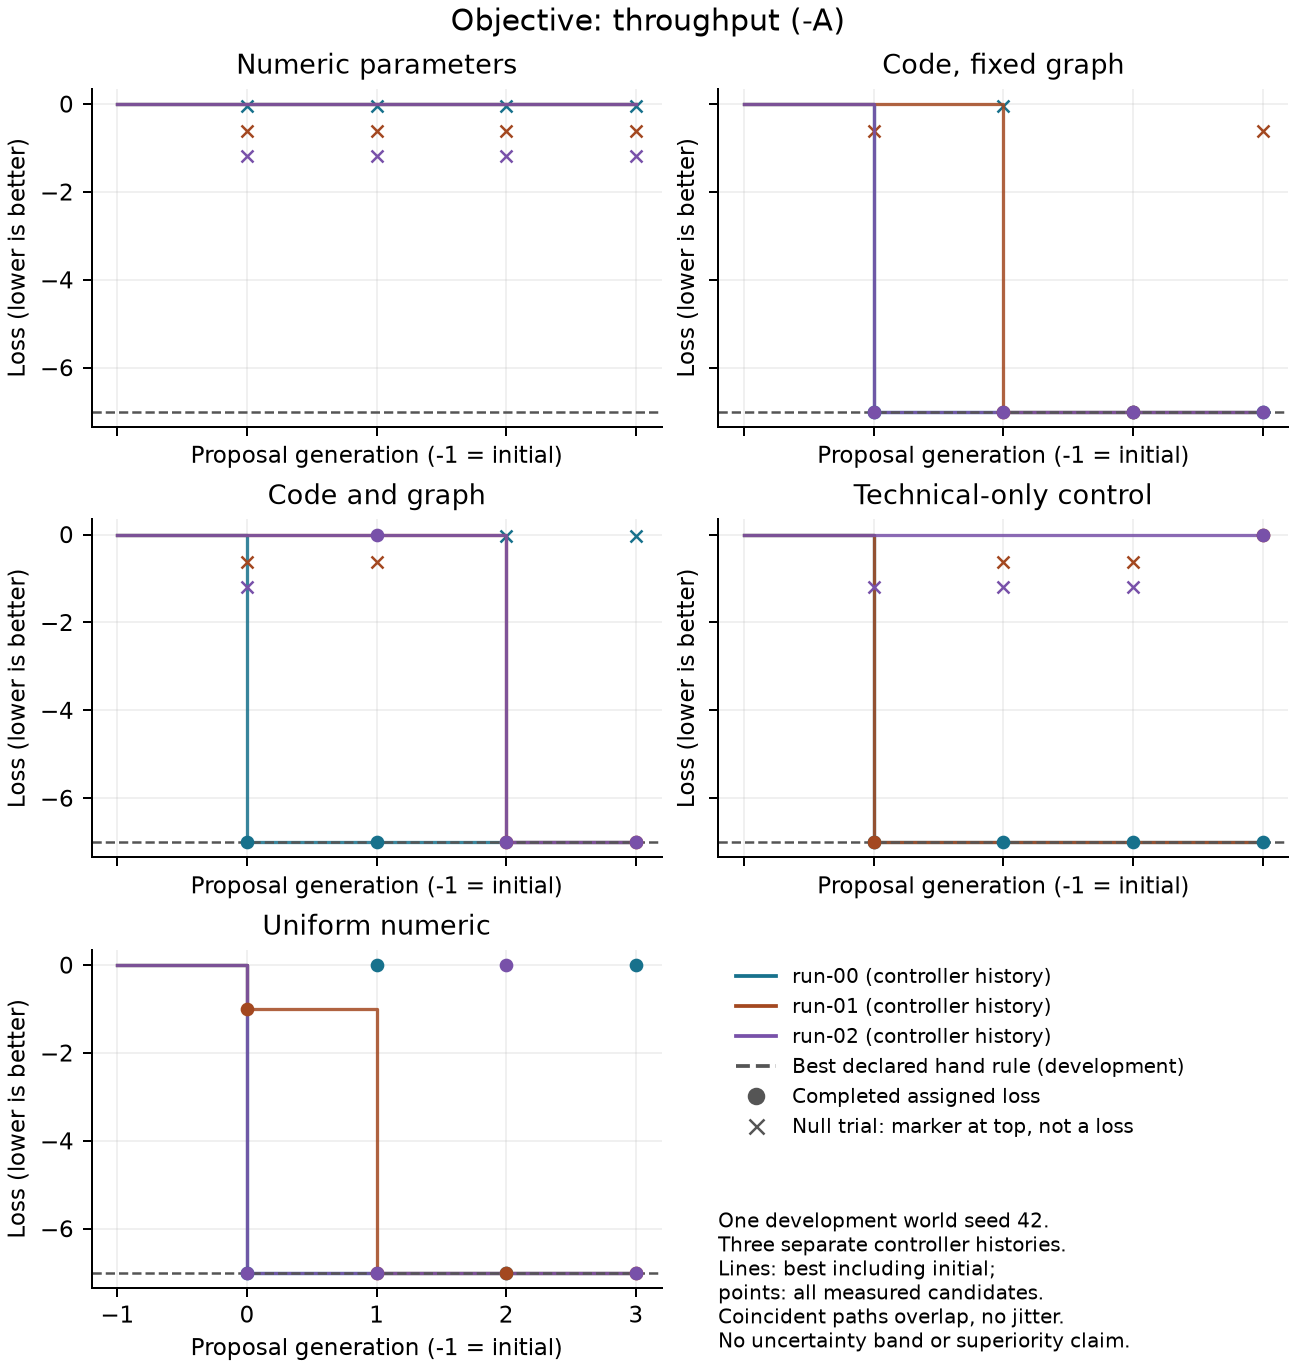
\includegraphics[width=\linewidth]{figures/native-design-v2/throughput-paths.png}
\caption{\textbf{All throughput development paths.} Four proposals per controller
history, all at world seed 42. Lines: best including initial; points: measured
candidates. Crosses at axes-relative positions are nulls, not loss penalties.
Coincident paths overlap without jitter. Dashed line: best declared hand rule.
Histories are not independent environment replicates.}
\label{fig:t-paths}\end{figure}
\begin{figure}[p]\centering
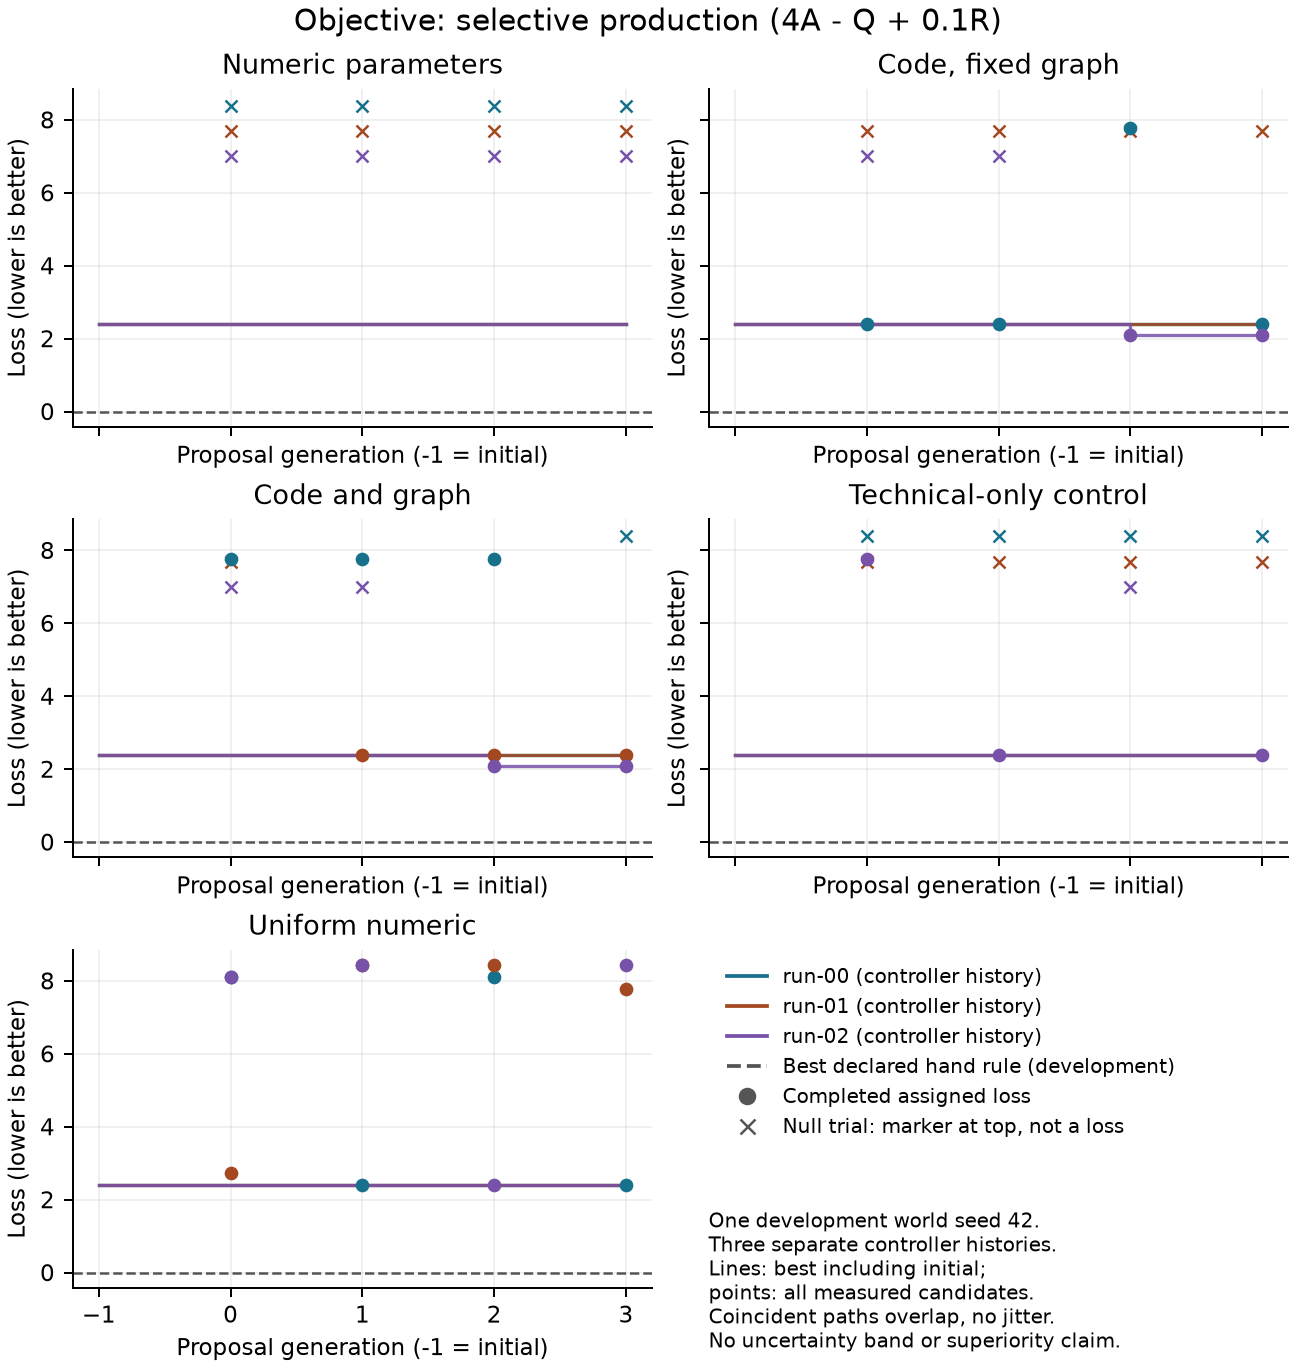
\includegraphics[width=\linewidth]{figures/native-design-v2/selective-paths.png}
\caption{\textbf{All review-cost-sensitive development paths.} Same full-budget
display for $C=4A-Q+0.1R$. Code proposals improve the weak initial proxy but not
reviewer-free reject 0. An incumbent line through a null is not a completed
trial. Permitted freedom does not isolate expressivity from interface compliance.}
\label{fig:c-paths}\end{figure}

\paragraph{Objective-conditioned outcomes.}
Figure~\ref{fig:cross} scores every reference and selection under common $T/C/E$.
Executable $T$ representatives and uniform selection accept mean 6.2 decisions
on five unused two-year seeds, matching the observed hand-written accept-all
and threshold 3 counts. Legacy averages 2.6, editable seed 0.2. Reviewer-free
accept-all also averages 6.2, but $Q=R=0$: a throughput tie is not equivalent
review-backed utility or better science. Both $C$ code selections have $A=Q=0$
and mean $R=19.2$, giving mean $C=1.92$. Editable seed and review-based reject-all
each have mean $C=2.58$; reviewer-free reject remains 0. Thus the gain is relative
to a cost-bearing reference, not the strongest simple policy. Diagnostic
mean $E=9.6$ is not favorable review-backed utility. Objective conditioning
selects different observed acceptance/review behavior, not a novel optimal policy.

\begin{figure}[p]\centering
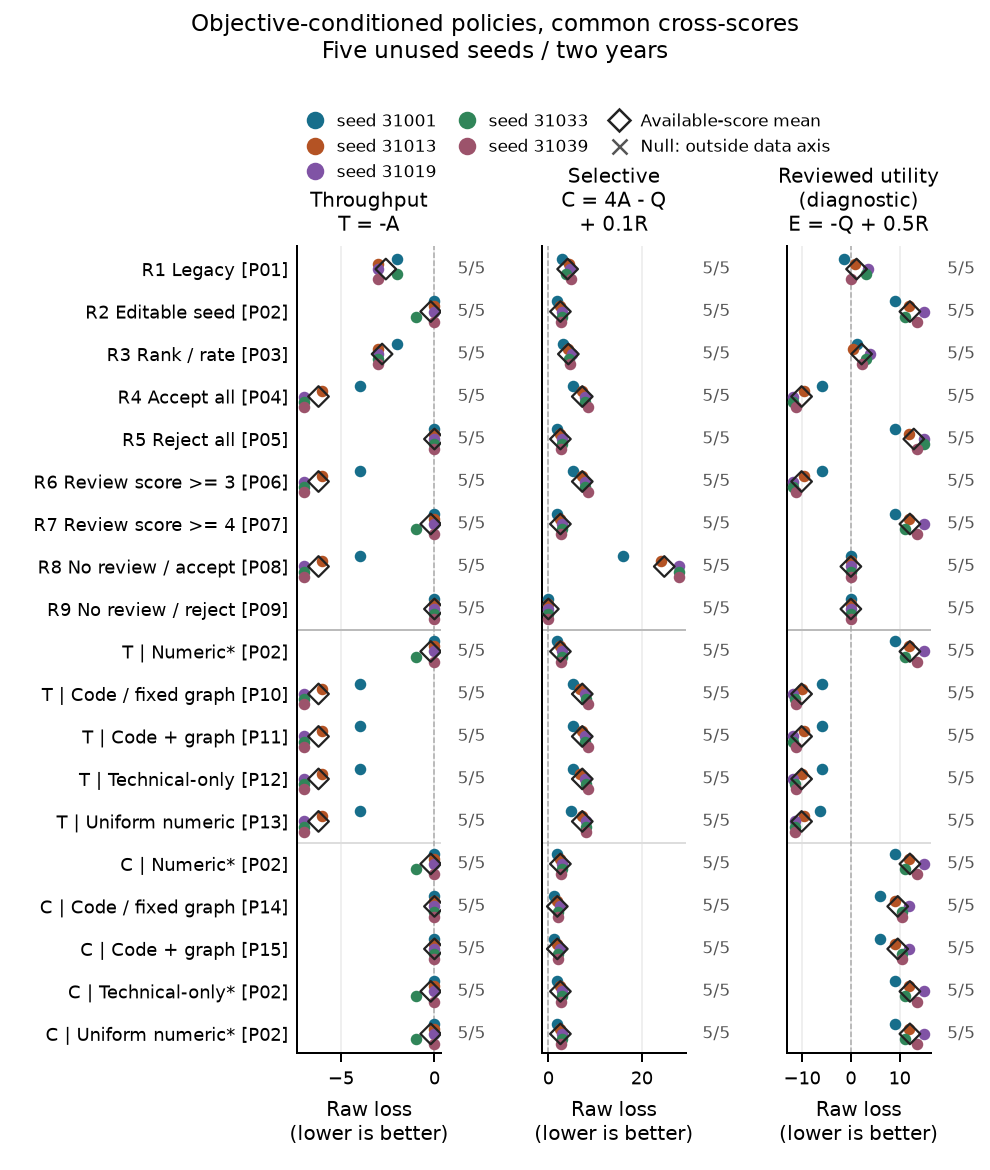
\includegraphics[width=\linewidth]{figures/native-design-v2/cross-objective-2y.png}
\caption{\textbf{Selection-fixed policies under common objectives.} All 9 references
and 10 arm selections receive three scores. Colored points: five raw seeds;
hollow diamonds: available-score means, not confidence intervals. Gutters:
$n/N$. T/C label the search objective; E is diagnostic. Separate raw loss scales,
no normalization or cross-loss ranking/averaging. P numbers identify shared exact
policies/jobs, not extra observations. Stars mark initial selections, not invented
replacements for failures. Four-year diagnostic: Appendix~\ref{sec:longer}.}
\label{fig:cross}\end{figure}

\section{Institutional mechanisms, not labels}
The development $C=2.1$ selections differ: code/graph has $A=Q=0,R=21$, while
fixed-graph has $A=1,Q=4,R=21$, where $4A-Q$ cancels. Authored final score 0 does
not set original-review measurement $Q$ to 0. Raw $A/Q/R$ and all ties matter
even when the primary loss is identical.

The selected $C$ code/graph program rejects real addressed papers and writes
score 0. The kernel stores it on the actual paper; publication commits it to
review history; the researcher resubmission prompt prints that history. In
its audited development world, three year 2 requests contain the corresponding
year 1 paper and score 0.00. Each joins one completed response declining
resubmission. This is an exercised \emph{program--record--researcher input--action}
path, not merely a fingerprint or designer explanation. It does not isolate
score 0 as the cause of fewer reviews: fresh LLM realizations are not perfectly
coupled and no alternate world is simulated. Unexercised dummy-ID/empty-input
branches are not validated by the successful trajectory.

One fixed-graph $C$ history's generations 2/3 have different source bytes but equal
Python ASTs and otherwise equal SystemSpecs. Both retain their costs and
physical evaluations; AST deduplication was not a selection rule. Conversely,
equal observed decisions do not prove equivalence on arbitrary inputs.
Source, consumers, receipts and downstream inputs are needed together.

Holding realized records/reviews fixed, accepting original score $q_i$ changes
$C$ by $4-q_i$, favoring rejection below 4. Removing review can reach $C=0$
without publication. For $A>0$, full-trajectory $C<0$ requires
$Q/A>4+0.1R/A$. This explains incentives, not a dynamic-policy bound: decisions
change future submissions and reviews. Fixed-record analysis has 163 complete
forwards and 56 unavailable identities, not 219 new/completed worlds.

\section{Related work and limitations}
The AI Economist learns social policies \citep{zheng2020economist}; AMD-LLM
evolves mechanism code with problem-specific fixing \citep{liu2025mechanism}.
No host repair here is a contract difference, not a performance advantage.
ADAS searches code-defined workflows \citep{hu2024adas}; OPRO uses evaluated
solutions \citep{yang2024opro}; SGA combines discrete LLM search and continuous
optimization \citep{ma2024sga}; GPTSwarm optimizes graph edges with REINFORCE
\citep{zhuge2024gptswarm}. These loops and estimators are prior art.
LLM Economist optimizes bounded tax actions over adapting workers
\citep{karten2025economist}; AgentSociety2 supports composable worlds and
specification-to-code \citep{piao2026agentsociety2}; SocialSystemArena compares
governance specifications \citep{fei2026institutions}; PolicySim optimizes
exposure actions \citep{huang2026policysim}. Our domain is executable organization
of persistent science, not just a fixed institution menu. Domain specificity
alone establishes neither generality nor algorithmic novelty.

This simulation uses one researcher model and one designer. It retrieves
literature instead of conducting physical experiments. Three histories are not three development
environments; five unused seeds remain small, and four years has one seed.
Scores do not measure true scientific quality. Interface/domain compliance
confounds expressivity; calibration does not establish task comprehension.
Useful graph invention, feedback/gradient superiority and inventor-weight
self-improvement are not demonstrated. The English game UI renders canonical
evidence, not a completed or user-evaluated management game. Reproduction,
compute and deployment limits follow below.

\section{Conclusion}
Scientific organization can be an executable optimization object without
training researcher weights or differentiating the entire world. Objectives
select different observed acceptance/review behavior, while strong simple
references remove apparent gains based on the editable seed alone. Graph
permission is not invention, failure is not a measured bad loss, and a scalar
tie is not one institutional mechanism. These distinctions make scientific-system
design testable without forcing positive results or recommending proxy optima
as science policy.

\bibliographystyle{plainnat}
\bibliography{references,submission-sources}
\appendix
\section{Four-year single-seed diagnostic}\label{sec:longer}
At seed 31001, throughput-selected executable policies, uniform tuning and
accept-all each produce 11 acceptances. Both $C$ code selections have $A=Q=0,R=33$,
giving $C=3.3$, versus editable seed 6.9 and reviewer-free reject 0. Diagnostic $E$
differs for some equal-throughput policies. This one fresh realization does not
establish a method/policy effect or another five-seed estimate.
\begin{figure}[p]\centering
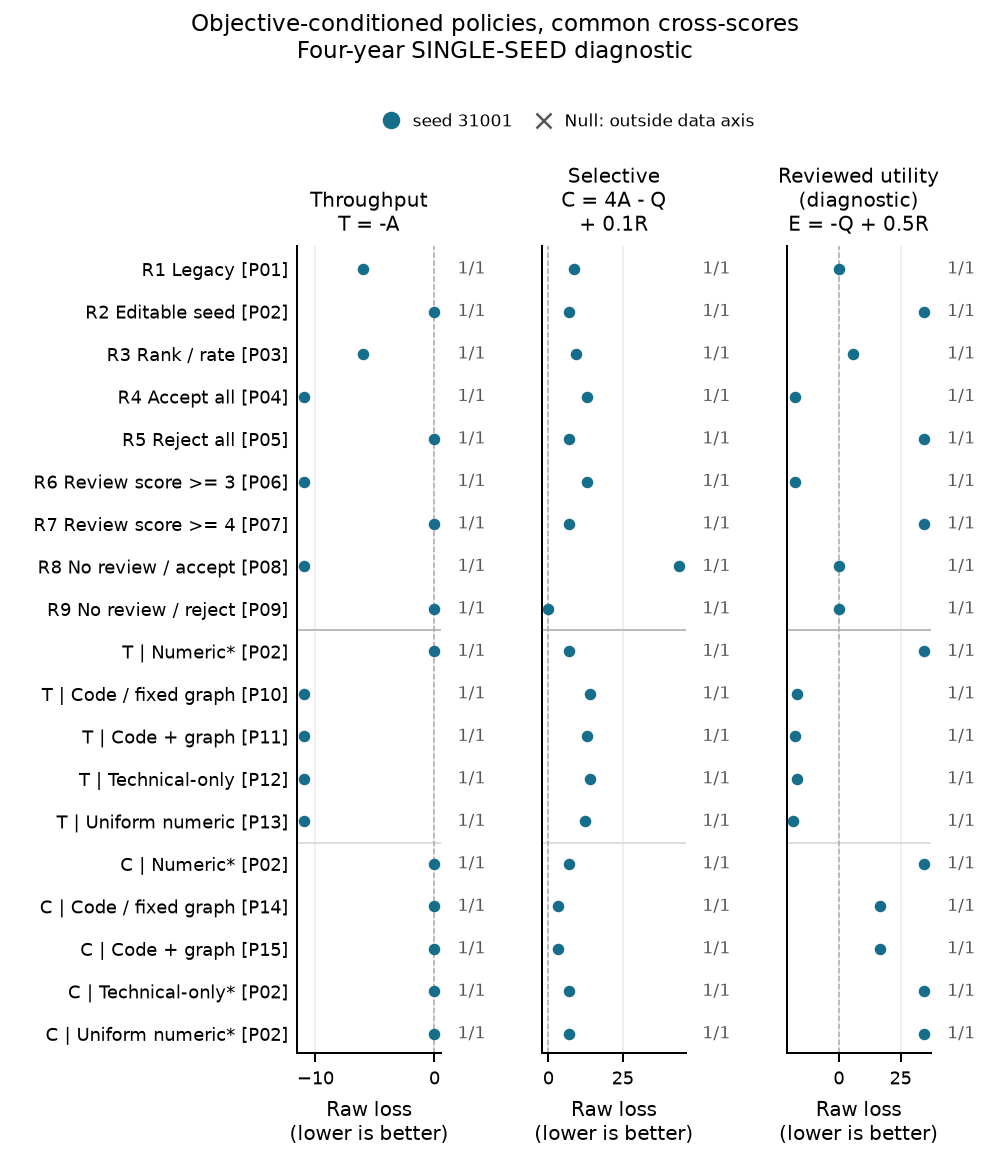
\includegraphics[width=\linewidth]{figures/native-design-v2/cross-objective-4y.png}
\caption{\textbf{Separate four-year diagnostic.} One seed; no confidence band
or redundant mean. Same labels, objectives and sharing as Figure~\ref{fig:cross}.
Gutters: $n/N$. P numbers: shared jobs, not independent observations. Stars:
initial selections. Separate raw scales; E remains diagnostic.}
\end{figure}

\section{Audit and reproduction boundary}
V2 source is \texttt{b6654adefc42223f9ecc}\allowbreak\texttt{7b4e53c043c879230f68}.
Two read-only audits are byte-identical, verifying 278 source and 7038 raw files
after normal closure. An explicit pinned adapter restores plan/selection mapping
order after sorted JSON, preserving values, hashes, list order and every original
guard. The unmodified frozen CLI is not claimed to pass; replaying one auditor
is not independent methodological validation or another scientific sample.

Numerical rebuilding, full raw re-audit and fresh inference are different
reproduction tiers. Raw journals/caches/checkpoints remain outside Git; compact
hashes/projections bind the paper. Seeds do not guarantee identical fresh replies.
The local 35B manifest/digest is retained, but its upstream revision/conversion
recipe is unknown; a public same-name tag has different tensor descriptors.
The alias suggests 64k while actual context is 40960. No weights are replaced;
complete fresh-machine inference reproduction is not established.

\section{Loss relaxation and domain diagnostic}
Freeze $N$ realized records, original means $q_i$ and review count $R$, with $q_i=0$
without review. For flags $z_i\in\{0,1\}$,
\begin{align}
 T_{\min}^{\rm rec}&=-N,&
 C_{\min}^{\rm rec}&=0.1R+\sum_i\min(0,4-q_i),&
 E_{\min}^{\rm rec}&=0.5R+\sum_i\min(0,-q_i).
\end{align}
Zero coefficients remain ties. Future histories are not replayed. Missing scores
can make this unavailable without invalidating an original loss; independent-sum
roundoff stays separate. No feasible-policy optimum or selection veto follows.

All 24 initial numeric-arm HTTP requests contain the correct six-coordinate
contract, with 12145--12411 native prompt tokens at 40960/8192 context/output and
no truncation. A general SYSTEM editor coexists with domain restrictions in
session data. Presence proves neither salience, later-call capacity nor cause.
All 25 generation-null slots lack valid explicit finish within 16 actions;
rejected output remains raw, without host repair or replacement.

\clearpage
\section{Resources and responsible interpretation}
\begin{table}[h]\centering\small
\begin{tabular}{@{}lrrr@{}}\toprule
Recorded stream & Responses & Input tokens & Output tokens\\\midrule
Scientists (including partial worlds)&16,043&15,547,758&1,473,665\\
Designer proposals&1,387&25,969,867&267,057\\
Designer calibration&84&808,832&3,819\\\bottomrule
\end{tabular}
\caption{\textbf{Measured response usage, not whole-project compute.} Input
includes cached subsets 2,976,386/3,102,175/22,464 respectively, never added
again. Aliases are not extra usage. Two proposal replies lack the declared
final-response signal; costs remain visible rather than assumed successful.}
\end{table}
Scientists have 194 physical journals, no unmatched wire input or missing/invalid
usage among 16,043 committed replies, and no provider total/component disagreements.
Their total is 17,021,423 tokens. Loads are separate: 99 designer/194 scientist
loads with unreported native usage unknown, not zero. Proposal/calibration/load
intents total 1764. Writer wall time is 21\,h\,55\,m\,58.697\,s. Host/provider/load/campaign
times overlap, not disjoint additive costs. Equal slots are not equal compute.

Post-dispatch observations report Apple M5 Pro, 18 logical CPUs, 64\,GiB memory
and Ollama 0.33.3, not startup attestation, serving-variant or GPU-use proof.
Caches, retrieval, containers, earlier development and coding/audit work are not
fully measured as FLOPs, energy or money. Separate earlier V1 (8 candidates,
4 runtime nulls) and S1 (8 developer rules) are not pooled as matched V2 outcomes.

No humans are recruited or real policy deployed. Publication/review proxies can
favor low activity or undesirable incentives. Reporting an optimum does not
recommend it or justify hiding it/adding a veto. The network-disabled container
has no host fallback, not proven immunity to all sandbox/kernel vulnerabilities.
Raw archives may contain literature text/author metadata; redistribution,
anonymous packaging and model release require separate review, not blanket
permission from public availability. Coding-agent assistance supports code,
analysis and drafting, not independent empirical validation. Human authorship
requires confirmation. The 2025 preprint style does not establish future-venue
compliance or actual submission.
\end{document}
